\documentclass[a4paper,12pt]{report}
%general packages
\usepackage[T2A]{fontenc}
\usepackage[utf8]{inputenc}
\usepackage[english,russian]{babel}
\usepackage{circuitikz}
\usepackage{wrapfig}
\usepackage{makecell}
\usepackage{tabularx}
\usepackage{graphicx}
\usepackage{gensymb}
\usepackage{cancel} %cancel symbol
\usepackage{amsmath,amsfonts,amssymb,amsthm,mathtools}
\usepackage[dvipsnames]{xcolor}


%\usepackage{epstopdf} %converting to PDF
%\usepackage{auto-pst-pdf}

%fancy header + geometry
\usepackage{fancyhdr}
\usepackage[a4paper,includehead,nomarginpar,left=15mm,right=15mm,top=15mm,headheight=10mm,bottom=20mm]{geometry}

%pgfplots
\usepackage{pgfplots}
\usepackage{pgfkeys}
\pgfplotsset{compat=1.12}
\usepackage{mathrsfs}

%multi column text
\usepackage{blindtext}
\usepackage{multicol}

%tikz (draw)
\usepackage{tikz}
\usepackage{pstricks-add}
\usetikzlibrary{intersections}
\usetikzlibrary{arrows.meta}
\usetikzlibrary{calc,angles,positioning}
\usetikzlibrary{arrows}
\usepackage{float}
\usepackage{filecontents}

%parskip settings
\parindent=0ex
\setlength{\parskip}{\baselineskip}%
\setlength{\parindent}{0pt}%

%fancy notation for sets
\newcommand{\R}{{\mathbb R}}
\newcommand{\N}{{\mathbb N}}
\newcommand{\fancy}[1]{{\mathbb{#1}}}
%sgn function
\DeclareMathOperator{\sgn}{sgn}

% intersection and union symbols
\newcommand{\uni}{\cup}
\newcommand{\inter}{\cap}
\newcommand{\re}{\text{Re}}
\newcommand{\const}{\text{const}}

\renewcommand{\footrulewidth}{0.4pt}

%\newcommand{\celsius}{$\ ^\circ C$}

%environments

\newtheorem{problem}{Задача}[]
\newenvironment{sol}{\paragraph{Решение}}{}
\renewcommand\thesection{\arabic{section}}

\usepackage{titlesec}
\titlespacing*{\section}
{0cm}{\baselineskip}{0pt}
\titlespacing*{\subsection}
{0pt}{0.1\baselineskip}{0.1\baselineskip}
\titlespacing*{\paragraph}
{0pt}{0.1\baselineskip}{\baselineskip}

\setcounter{secnumdepth}{0}

\begin{document}
	

\begin{titlepage}
	\begin{center}
		МОСКОВСКИЙ ФИЗИКО-ТЕХНИЧЕСКИЙ ИНСТИТУТ (НАЦИОНАЛЬНЫЙ ИССЛЕДОВАТЕЛЬСКИЙ УНИВЕРСИТЕТ) \\
		
		
		\hfill \break
		Факультет обшей и прикладной физики\\
		\vspace{2.5cm}
		\large{\textbf{Отчёт по лабораторной работе 1.2.5 <<Исследование прецессии уравновешенного гороскопа>>}}\\
		\hfill \break
		\\
	\end{center}
	
	\begin{flushright}
		Выполнил:\\
		Студент гр. Б02-304\\
		Головинов. Г.А.
	\end{flushright}
	
	\vspace{7cm}
	
	\begin{center}
		
\includegraphics[width=0.15\linewidth]{uni}
	\end{center}
	

	

	\vfill
	
	\begin{center} Долгопрудный, 2023 \end{center}
	
	\thispagestyle{empty}
	
\end{titlepage}


	\newpage
	%\pagenumbering{arabic}
    \pagestyle{fancy}

    \fancyhead{}
    \fancyfoot{}
    \fancyhead[L]{\rightmark}
    \fancyhead[R]{\thepage}
    \fancyfoot[R]{Работа 2.3.1. --- получение и измерение вакуума}

    \section*{Аннотация}
        \paragraph*{Цель работы:} 1) измерение объёмов форвакуумной и высоковакуумной частей установки; 2) определение скорости откачки системы в стационарном режиме, а также по ухудшению и улучшению вакуума.
        \paragraph*{В работе используются:} вакуумная установка с манометрами: масляным, термопарным и ионизационным.
    \vspace{0.5cm}
    \hrule

    \section{Основные теоретические сведения}

    \subsection{Принцип работы ионизационного манометра}

    \begin{multicols}{2}
        Ионизационный манометр представляет собой трёхэлектродную лампу. Электроны испускаются накалённым катодом и увлекаются электрическим полем к аноду. Проскакивая за витки анода, электроны замедляются полем коллектора и возвращаются к катоду, а от него вновь увлекаются к аноду.

        Перед тем, как осесть на аноде они успевают много раз пройти расстояние между катодом и анодом, на этом пути они ионизируют молекулы газа. Ионы, образовавшиеся между анодом и коллектором, притягиваются его полем. По ионному току в цепи можно понять плотность молекул газа (она пропорциональна току), отсюда уже можно найти давление газа. 

        \begin{figure}[H]
            \centering
            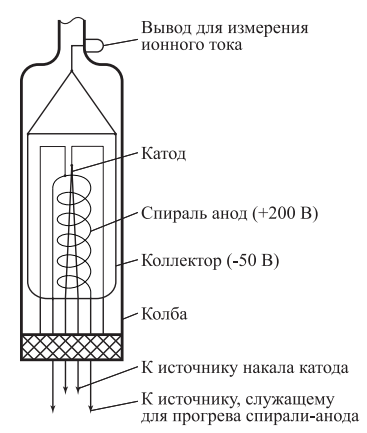
\includegraphics[width=0.7\columnwidth]{../img/ion_lamp.png}
            \caption{Схема ионизационной лампы.}
        \end{figure}
    \end{multicols}

    \hrule

    \begin{figure}[H]
        \centering
        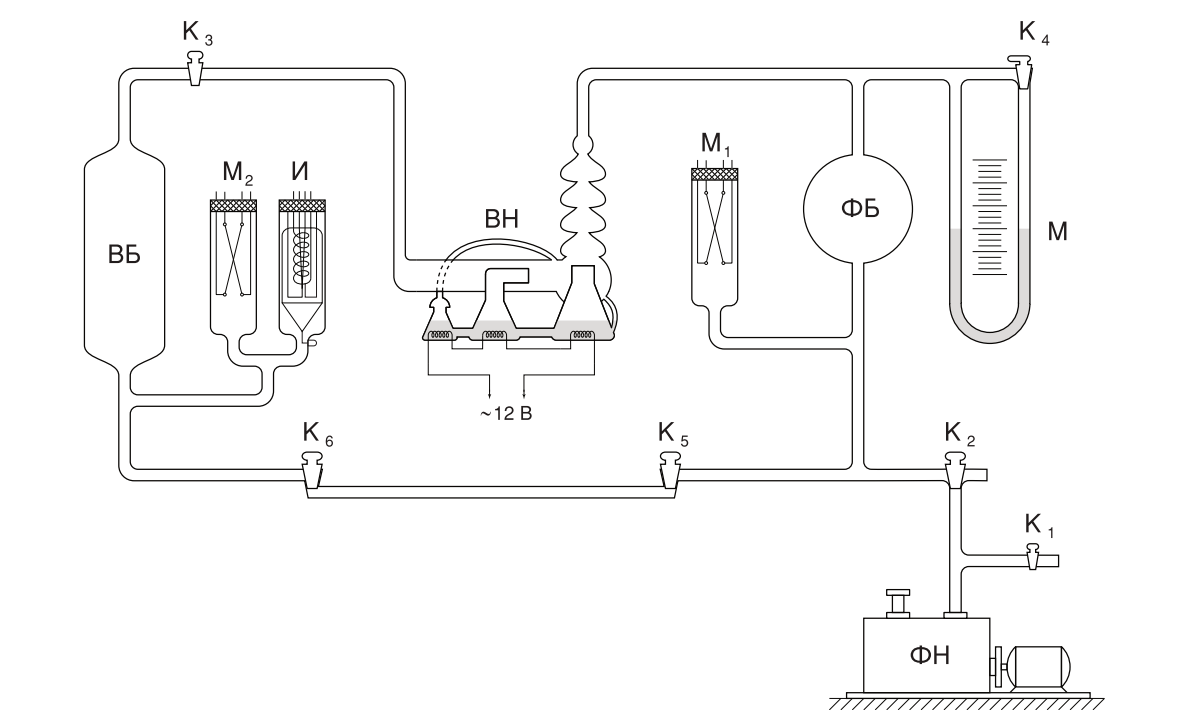
\includegraphics[width=0.5\linewidth]{../img/ustanovka.png}
        \caption{Схема Экспериментальной установки.}
    \end{figure}

    \newpage

    \subsection{Процесс откачки}

    \begin{multicols}{2}
        Пусть $W$ --- скорость откачки насосом, $Q_\text{д}$ --- количество газа, десорбирующегося с поверхности откачиваемого объема в единицу времени, $Q_\text{и}$ --- количество газа, проникающего в единицу времени извне, $Q_\text{н}$ --- поток газа, поступающего обратно из насоса. Все потоки $Q$ будем измерять в единицах $pV$.

        \begin{gather}
            -Vdp=(pW-Q_\text{д}-Q_\text{н}-Q_\text{и})dt \label{eq:1}
        \end{gather}

        При достижении предельного давления $p_\text{пр}$:
        \begin{gather*}
            \frac{dp}{dt}=0
        \end{gather*}
        значит
        \begin{gather}
            p_\text{пр}W=Q_\text{д}+Q_\text{н}+Q_\text{и}
            \label{lim}
        \end{gather}

        Обычно $Q_\text{и}$ --- постоянно, а два других потока слабо зависят от времени, поэтому скорость откачки $W$ можно считать постоянной. Чтобы отойти от предельного давления следует проинтегрировать \eqref{eq:1}:

        \begin{gather*}
            -V\int_{p_\text{пр}}^{p}\frac{dp}{p}=\int_{0}^{t}\left(W-\frac{\sum Q_i}{p}\right)dt \\
            p-p_\text{пр}=(p_0-p_\text{пр})\exp{\left(-\frac{W}{V}t\right)}
        \end{gather*}
        Будем тогда аппроксимировать функцией:

        \begin{gather}
            p(t)=p_1 \exp\left(-\frac{W}{V}t\right)+p_2
        \end{gather}
        где $p_1=p_0-p_\text{пр}$, $p_2=p_\text{пр}$.

    \end{multicols}

    \hrule

    \section{Обработка результатов измерений}

    \begin{multicols}{2}
        С помощью капилляра известного объема, кранов и масляного манометра определим объем вакуумной и форвакуумной части установки:

        \begin{gather*}
            V_\text{форвакуумной}=2110 \  \text{см}^3\\
            V_\text{вакуумной}=1141 \ \text{см}^3
        \end{gather*}

        После достижения $3\cdot 10^{-2}$ торр начинаем высоковакуумную откачку с помощью диффузионного насоса. При достижении $7\cdot 10^{-4}$ торр на термопарном манометре включаем ионизационную лампу. Ждем установления предельного давления. В нашем случае оно составило $2\cdot 10^{-4}$ торр.

        Закрывая и открывая кран, ведущий к диффузионному насосу, оценим ухудшение и улучшение вакуума:

        \begin{figure}[H]
            \centering
            \begin{tikzpicture}[scale=0.9]
                \begin{axis}[name=plot1,
                    title={Ухудшение давления в высоковакуумной части},
                    xlabel={$t$, c},
                    ylabel={$p$, $\cdot$10$^{-4}$ торр},
                    legend pos=north west,
                    ymajorgrids=true,
                    xmajorgrids=true,
                    grid style=dashed,]
                    \addplot[line width=1pt,solid,color=blue] %
                    table[x=t,y=p,col sep=comma]{../data/bad.csv};
                    \addlegendentry{$p(t)$}
                    \addplot[black,dashed,domain=7:34] {0.163*x+0.55};
                    \addlegendentry{Аппроксимация}
                \end{axis}
            \end{tikzpicture}
            \caption{Ухудшение давления со временем из-за течи в системе.}
            \label{fig:1}
        \end{figure}

        \begin{figure}[H]
            \centering
            \begin{tikzpicture}[scale=0.9]
                \begin{axis}[name=plot1,
                    title={Улучшение давления в высоковакуумной части},
                    xlabel={$t$, c},
                    ylabel={$p$, $\cdot$10$^{-4}$ торр},
                    legend pos=north east,
                    ymajorgrids=true,
                    xmajorgrids=true,
                    grid style=dashed,]
                    \addplot[line width=1pt,solid,color=blue] %
                    table[x=t,y=p,col sep=comma]{../data/good.csv};
                    \addlegendentry{$p(t)$}
                    \addplot[black,dashed,domain=0:14] {7.15*e^(-x/4.88)+1.13};
                    \addlegendentry{Аппроксимация}
                \end{axis}
            \end{tikzpicture}
            \caption{График улучшения давления при работающем диффузионном насосе.}
        \end{figure}

        Аппроксимируя по методу $\chi^2$ получим характерное значение $\tau = (4.88\pm 0.29) \ \text{с}$. При этом $p_1 = (7.15\pm 0.07)$ Па, $p_2 = (1.12 \pm 0.10)$ Па.

        Из него получим по формуле $\tau = V/W$:
        \begin{gather*}
            W=(233.8 \pm 13.9) \ \text{см}^3/\text{с}
        \end{gather*}

        Получим величину откачки другим образом: сделаем искусственную течь. Установившееся давление при этом равно $2.9\cdot 10^{-4}$ торр.
        
        \begin{gather*}
            W(p_\text{уст}-p_\text{пр})=\frac{d(pV)_\text{капилляра}}{dt} \\
            W=\frac{4}{3}\frac{r^3}{L}\sqrt{\frac{2\pi R T}{\mu}}\cdot\frac{p_\text{фв}}{p_\text{уст}-p_\text{пр}}
        \end{gather*}

        Учитывая давление в форвакуумной части $p_\text{фв}$ получим $W\approx 290 \ \text{см}^3/\text{с}$, что несколько больше $W$ из аппроксимации. Это может быть связано с тем, что в установке появились новые течи, а также с тем, что в реальности $W$ все же зависит от давления.
        
        Теперь оценим величину $Q_\text{н}$. Это можно сделать следующим образом:

        Из \ref{fig:1} найдем наклон прямой: $V\cdot dp/dt=Q_\text{и}+Q_\text{д}$. $Q_\text{н}$ свой вклад в данном случае не вносит, так как насос не имеет доступа к высоковакуумной части установки в это время.

        Тогда используя формулу \eqref{lim} найдем $Q_\text{н}$:
        \begin{gather}
            Q_\text{н}=p_\text{пр}W-(Q_\text{и}+Q_\text{д})=p_\text{пр}W-V\cdot \frac{dp}{dt}
        \end{gather}

        Точки достаточно хорошо ложатся на прямую, коэффициент $k=dp/dt\approx 0.16\cdot 10^{-4}$ торр/с. Получим:
        \begin{gather*}
            Q_\text{н}=(280.7\pm 16.7)\  \text{торр}\cdot\text{см}^3/\text{с}
        \end{gather*}
    \end{multicols}

    \hrule

    \section{Выводы}

    \begin{multicols}{2}
        В результате работы мы познакомились с методами получения и измерения вакуума, с помощью диффузионного насоса получили довольно высокий вакуум, исследовали характеристики насоса при этих давлениях двумя методами. Сравнили результаты.

        Значения несколько расходятся, это может быть объяснено в том числе тем, что производительность насоса зависит от давления.
    \end{multicols}
\end{document}
